% Compile with XeLaTeX + Biber in Overleaf.
\documentclass[12pt,a4paper]{article}

\usepackage[a4paper,margin=2.5cm]{geometry}
\usepackage{fontspec}
\IfFontExistsTF{Times New Roman}
  {\setmainfont{Times New Roman}}
  {\setmainfont{TeX Gyre Termes}} % Times-compatible fallback available in Overleaf
\usepackage{polyglossia}
\setdefaultlanguage{english}
\usepackage{microtype}
\usepackage{graphicx}
\usepackage{booktabs}
\usepackage{tabularx}
\usepackage{longtable}
\usepackage{array}
\usepackage{float}
\usepackage{amsmath}
\usepackage{caption}
\usepackage{enumitem}
\usepackage[hidelinks]{hyperref}
\usepackage[style=apa,backend=biber]{biblatex}
\DeclareLanguageMapping{english}{english-apa}
\addbibresource{references.bib}

\newcolumntype{Y}{>{\raggedright\arraybackslash}X}
\newcommand{\projecttitle}{Anime Recommendation System}
\newcommand{\memberone}{Mai Nam Quốc -- 29211145181}
\newcommand{\membertwo}{Trương Nhật Trường -- 29211164915}


% Keep full identities on the cover, but use concise names in body text.
\let\memberonefull\memberone
\let\membertwofull\membertwo
\renewcommand{\memberone}{Quốc}
\renewcommand{\membertwo}{Trường}

\title{\projecttitle}
\author{Group 14}
\date{July 2026}

\begin{document}

\begin{titlepage}
  \centering
  {\Large \textbf{DUY TAN UNIVERSITY, DA NANG}\par}
  \vspace{1.2cm}
  {\large DS 423 --- Machine Learning with Large Datasets\par}
  \vspace{2.0cm}
  {\LARGE \textbf{\projecttitle}\par}
  \vspace{1.4cm}
  {\large Group 14\par}
  \vspace{1.2cm}

  \vspace{0.9cm}
  {\large \textbf{Individual contribution}\par}
  \vspace{0.35cm}
  \small
  \begin{tabularx}{\linewidth}{p{0.24\linewidth}Yc}
    \toprule
    \textbf{Member} & \textbf{Primary contribution} & \textbf{Share} \\
    \midrule
    \memberonefull & Dataset loading, data cleaning and preprocessing, EDA charts, data preparation, APA reference compilation, and report review. & 50\% \\
    \membertwofull & SVD model selection and implementation, evaluation, Top-10 export, presentation preparation, report integration, and conclusion drafting. & 50\% \\
    \bottomrule
  \end{tabularx}
  \par
  \vspace{0.25cm}
  \par
  \vfill
  \vspace{0.8cm}
  {\large July 2026\par}
\end{titlepage}

\begin{abstract}
Anime catalogues are large enough that manually finding titles aligned with a viewer's preferences is difficult. This project builds a collaborative-filtering recommender that estimates a user's preference for unseen anime and returns a Top-10 list. The Anime Recommendations Database provides 7,813,737 user--anime interactions and title metadata. Data preparation removed 1,476,496 watched-but-unrated records encoded as $-1$, merged seven repeated user--anime pairs, and retained 6,337,234 valid explicit ratings on the original 1--10 scale. The resulting matrix is sparse (0.9172\%), with positively skewed ratings and highly unequal user histories.

For a reproducible resource-aware experiment, the modeling notebook randomly sampled one million cleaned ratings, applied a minimum-five-interaction k-core filter, and trained a biased SVD model on an 80/20 outer holdout split. A validation split inside the outer training data selected 30 latent factors from the candidates 30, 50, and 100. The resulting model obtained RMSE 1.2551, MAE 0.9560, Precision@10 0.6397, and Recall@10 0.8273 under held-out observed-item ranking. These results describe the sampled and filtered evaluation population, rather than the whole catalogue. The system cannot fully address new users or new anime, and observed-item ranking is not equivalent to full-catalog ranking.
\end{abstract}

\section{Project approach and team workflow}
The group treated the recommender as a sequence of evidence-based decisions rather than as a single SVD training task. The initial question was whether the raw interaction table contained a valid preference signal; only after that question was answered did the group choose a model and an evaluation protocol. Table~\ref{tab:team-workflow} records the reasoning chain, the ownership of each stage, and the artifact handed to the next stage. It therefore distinguishes the audited cleaned dataset from the smaller, model-specific dataset and distinguishes evaluation from the final recommendation-serving step.

\begin{table}[H]
  \centering
  \caption{Team workflow: decision sequence, rationale, and handoff artifacts.}
  \label{tab:team-workflow}
  \small
  \begin{tabularx}{\linewidth}{p{0.16\linewidth}Y Y p{0.18\linewidth}}
    \toprule
    \textbf{Stage} & \textbf{Question and decision} & \textbf{Reasoning and output} & \textbf{Lead / review} \\
    \midrule
    Define the task & What should be predicted and ranked? The group used explicit 1--10 user ratings to estimate preferences for unseen anime. & Missing interactions were treated as unknown rather than zero or negative ratings. This fixed the target, candidate meaning, and Top-10 objective. & Both define; \membertwo integrates \\
    Audit and prepare data & Which rows are valid learning signals? Remove the watched-but-unrated sentinel $-1$, validate the 1--10 scale, and merge repeated user--anime pairs by their mean. & The resulting \texttt{ratings\_clean.csv} preserves only explicit preferences and gives Notebook 02 a reproducible, auditable input. & \memberone leads; \membertwo checks boundary \\
    Examine data reality & What constraints should influence modelling? Measure sparsity, rating skew, popularity concentration, and unequal user histories. & EDA showed a sparse, positive, long-tail matrix; it motivated collaborative filtering, explicit coverage reporting, and careful interpretation rather than an assumption that all users have equal evidence. & \memberone leads; both review \\
    Model and test & How can the system be trained and assessed without leakage? Use a fixed-seed sample and k-core filter, then an outer 80/20 holdout and biased SVD fitted on training data only. & Notebook 02 records configuration, data scope, RMSE/MAE, and held-out observed-item Precision@10/Recall@10. & \membertwo leads; \memberone verifies inputs/results \\
    Serve and integrate & How are recommendations made useful without changing the test result? Refit the fixed SVD on all model-scope interactions and rank only unseen candidates. & The export, report, figures, references, and presentation were cross-checked so that claims, metrics, and contribution shares remain consistent. & \membertwo leads serving/report integration; both review \\
    \bottomrule
  \end{tabularx}
\end{table}

\subsection{Data and analysis approach: \memberone}
The data-and-analysis work began by separating a data-quality question from a modelling question. Before deciding how to train a recommender, \memberone established what a valid user-preference observation meant and whether the raw files could support that meaning. The process was deliberately ordered: inspect first, define each cleaning rule from the meaning of the data, validate the resulting table, then use EDA to identify constraints that the later model must disclose. This avoided treating routine data transformations as assumptions hidden inside model code. Table~\ref{tab:memberone-process} gives the detailed decision record.

\begingroup
\small
\begin{longtable}{@{}p{0.12\linewidth}@{\hspace{0.8em}}p{0.24\linewidth}@{\hspace{0.8em}}p{0.32\linewidth}@{\hspace{0.8em}}p{0.22\linewidth}@{}}
  \caption{Detailed decision record for the data and EDA work led by \memberone.}\label{tab:memberone-process} \\
    \toprule
    \textbf{Step} & \textbf{Evidence examined} & \textbf{Decision logic and action} & \textbf{Output / handoff} \\
    \midrule
    \endfirsthead
    \multicolumn{4}{@{}l}{\small\itshape Table~\ref{tab:memberone-process} continued} \\
    \toprule
    \textbf{Step} & \textbf{Evidence examined} & \textbf{Decision logic and action} & \textbf{Output / handoff} \\
    \midrule
    \endhead
    \midrule
    \multicolumn{4}{r@{}}{\small\itshape Continued on next page} \\
    \endfoot
    \bottomrule
    \endlastfoot
    1. Establish the raw-data boundary & The two source tables and their required fields: user ID, anime ID, rating, and display metadata. & Read IDs without assuming they are numeric features; keep ratings observable until parsing so a malformed value cannot silently become a valid score. Verify schema, completeness, parseability, candidate-key duplicates, and metadata coverage before altering rows. & A before-cleaning quality snapshot for \texttt{rating.csv} and \texttt{anime.csv}. \\
    2. Define a valid rating signal & The raw rating range and the 1,476,496 rows encoded as $-1$. & Interpret $-1$ from the dataset semantics as ``watched but not explicitly scored.'' It gives no numerical preference direction, so retaining it would teach SVD that an unknown preference is worse than rating 1. Exclude it from both training and evaluation instead of converting it to zero or one. & An auditable removal count and a retained explicit 1--10 signal. \\
    3. Resolve interaction ambiguity & Repeated \texttt{(user\_id, anime\_id)} keys after valid ratings were isolated. & A matrix factorisation model needs one target value per user--anime pair. Average the seven duplicate pairs rather than arbitrarily keeping the first or last row; accept fractional averages only because they remain inside the valid 1--10 range. & \texttt{ratings\_clean.csv} with unique user--anime keys and scale assertions. \\
    4. Preserve the metadata boundary & Metadata IDs, missing display fields, and one rated anime without matching metadata. & Keep metadata for title/genre display only. Do not impute missing labels or use public \texttt{anime\_average\_rating} as a training label, because doing either would blur catalogue context with a user's explicit score. Retain valid ratings even when a display fallback will be needed later. & \texttt{anime\_clean.csv}, an unmatched-metadata audit, and a clear serving fallback requirement. \\
    5. Test the cleaned result & Counts, rating bounds, duplicate keys, and the post-cleaning user--anime matrix. & Use assertions to verify that no $-1$, missing required value, out-of-range rating, or duplicate interaction remains. This confirms that the cleaned table is a reproducible baseline rather than an informal spreadsheet edit. & 6,337,234 explicit interactions, 69,600 users, 9,927 rated anime, and a 0.9172\% matrix-density measurement. \\
    6. Translate EDA into modelling constraints & Rating distribution, title activity, and user-history distribution. & Read the mean 7.81/mode 8 and 82.55\% of ratings at least 7 as positive-score skew; read the median/P90/P99 user histories of 45/230/640 as unequal evidence; and read popularity concentration as a risk of uneven item support. These are reasons to report coverage and limitations, not reasons to delete active users or infer genre preferences. & Three EDA figures plus a written handoff specifying the original scale, missing-as-unknown rule, and coverage reporting. \\
\end{longtable}
\endgroup

The most consequential decision in this stage was the treatment of $-1$. If it had been kept as a numerical target, the model could confuse a user who simply did not score a watched title with a user who strongly disliked it. Conversely, removing it does not claim that the user disliked the title; it declares that this project uses explicit ratings only. The duplicate rule followed the same principle: the average preserves the available explicit information while ensuring one target per matrix cell. No missing or unparseable required explicit ratings and no invalid 1--10 ratings were removed, so the change log explains exactly why the raw total fell from 7,813,737 to 6,337,234.

The next step was to ask what the cleaned matrix implied for the rest of the project. The rating distribution established that explicit scores are concentrated at the high end; the user-activity distribution established that histories are long-tailed; and the density calculation established that almost all user--anime pairs are unobserved. From these observations, the handoff to modelling specified three constraints: preserve the original 1--10 scale, report the coverage effects of any sample or minimum-interaction rule, and do not turn missing entries into zeros. The cleaned CSV files, validation assertions, change log, and EDA figures are the concrete handoff artifacts from this approach.

\subsection{Modelling and evaluation approach: \membertwo}
The modelling work converted the data handoff into a reproducible recommendation experiment. \membertwo first kept the data boundary visible: \texttt{ratings\_clean} is the audited source from the first notebook, while \texttt{ratings\_model} is a resource-aware subset created only for SVD. The method was selected only after considering the task and EDA together. The task requires estimating a user's unseen-item preferences from explicit ratings, and the sparse matrix contains shared user--anime patterns that collaborative filtering can exploit. Biased SVD was therefore a direct, interpretable baseline; its latent factors are learned preference patterns, not manually named genres. Table~\ref{tab:membertwo-process} records the detailed sequence.

\begingroup
\small
\begin{longtable}{@{}p{0.12\linewidth}@{\hspace{0.8em}}p{0.24\linewidth}@{\hspace{0.8em}}p{0.32\linewidth}@{\hspace{0.8em}}p{0.22\linewidth}@{}}
  \caption{Detailed decision record for the SVD, evaluation, and serving work led by \membertwo.}\label{tab:membertwo-process} \\
    \toprule
    \textbf{Step} & \textbf{Evidence examined} & \textbf{Decision logic and action} & \textbf{Output / handoff} \\
    \midrule
    \endfirsthead
    \multicolumn{4}{@{}l}{\small\itshape Table~\ref{tab:membertwo-process} continued} \\
    \toprule
    \textbf{Step} & \textbf{Evidence examined} & \textbf{Decision logic and action} & \textbf{Output / handoff} \\
    \midrule
    \endhead
    \midrule
    \multicolumn{4}{r@{}}{\small\itshape Continued on next page} \\
    \endfoot
    \bottomrule
    \endlastfoot
    1. Recheck the modelling input & The cleaned schemas, scale, sentinel removal, duplicate-key condition, and metadata role. & Treat Notebook 01 as the only source of model input and revalidate it on load. This prevents a local manual change or an incorrect raw file from silently changing the experiment. Keep metadata out of SVD fitting and reserve it for readable recommendation output. & Validated \texttt{ratings\_clean} and \texttt{anime\_clean} inputs. \\
    2. Choose model scope and method & The 6.3-million-row cleaned dataset, sparse EDA results, and personal-computer resource limits. & Use deterministic sampling of 1,000,000 ratings with seed 42, followed by iterative user/item k-core filtering at five interactions. Choose biased SVD because it estimates explicit ratings from observed collaborative patterns without treating missing cells as zero. & \texttt{ratings\_model}: 952,497 interactions, 41,370 users, and 5,985 anime; an explicit scope limitation. \\
    3. Protect the holdout experiment & The risk that test ratings could influence fitted parameters or configuration decisions. & Split the filtered data once into 80\% training and 20\% outer test data before fitting. Within the outer training data only, compare 30-, 50-, and 100-factor SVD candidates on a seeded validation split; retain the best validation configuration. The outer test set remains untouched until final scoring. & 761,997 training ratings, 190,500 held-out ratings, and selected 30-factor SVD configuration. \\
    4. Measure two different questions & Outer-holdout predictions containing true and estimated ratings for each observed test item. & Compute RMSE and MAE for rating-estimation error. Separately rank each user's held-out predictions; define relevance as a true rating at least 8; require at least ten test items and one relevant item; then macro-average Precision@10 and Recall@10. This prevents a rating-error score from being mistaken for a Top-N retrieval score. & RMSE 1.2551, MAE 0.9560, Precision@10 0.6397, Recall@10 0.8273 for 4,802 eligible users. \\
    5. Bound metric interpretation & The candidate set and excluded users in the ranking calculation. & Label ranking evaluation as held-out observed-item ranking, not full-catalog ranking. Users without enough test items or without a relevant held-out item are excluded under the stated rule rather than assigned artificial zero recall. Record that the random split is not temporal forecasting. & Metric charts, eligibility counts, and limitations included with results. \\
    6. Separate evaluation from serving & The need for a final Top-10 list after the test metrics have been fixed. & Refit the same configuration on all \texttt{ratings\_model} interactions only after evaluation. For each selected demonstration user, exclude every already rated model-scope anime, predict the remaining candidates, use deterministic tie-breaking, then join metadata after ranking. & \texttt{top\_10\_recommendations.csv} and seven reproducible demonstration profiles. \\
\end{longtable}
\endgroup

The resource-aware filtering was a modelling choice, not a claim that sparse users or anime are invalid. Sampling made the run feasible, while the iterative k-core rule ensured that every retained user and anime had minimum local evidence after the mutual removals stabilised. Its cost is a narrower evaluation population, which is why every result is tied to the 952,497-interaction model dataset rather than the full cleaned catalogue. A lightweight validation search compared only 30, 50, and 100 latent factors; it is reproducible but not an exhaustive hyperparameter search.

The evaluation reasoning then separated an honest test from a usable serving model. An outer 80/20 split was created before SVD fitting; configuration selection used a further seeded split of the outer training data, so held-out ratings were not used to fit parameters or choose 30 latent factors. RMSE and MAE answer how close estimated ratings are to held-out ratings, whereas Precision@10 and Recall@10 answer whether relevant held-out observations are retrieved near the top under a documented observed-item protocol. Once those metrics were fixed, a separate model was refitted on all \texttt{ratings\_model} interactions to score only anime that a demonstration user had not rated. This sequence prevents the displayed Top-10 lists from being confused with test-set evidence, future verified ratings, or objective measures of anime quality.

\subsection{Shared integration and review}
The two workflows meet at explicit review checkpoints rather than only at the final writing stage. First, \membertwo accepts the cleaned files only after the scale, sentinel, duplicate, and metadata assertions from Notebook 01 pass. Second, \memberone reviews the post-sampling and post-filtering counts so the report never calls \texttt{ratings\_model} the entire dataset. Third, both members compare every reported number with the notebook-generated artifacts: cleaning counts and EDA summaries come from Notebook 01; configuration, split sizes, eligible-user counts, metrics, and Top-10 exports come from Notebook 02. This makes the notebook boundary a reproducibility control, not simply a division of labour.

For report integration, the group used a final claim-by-claim check. Public \texttt{anime\_average\_rating} remains display metadata and is never described as an SVD label or a personalised prediction. Figures are accompanied by an interpretation and a next-decision implication; metrics state their direction, data scope, and ranking protocol; and the conclusion does not generalise beyond the sampled, k-core-filtered, random-holdout experiment. Both members also verified that the contribution shares total 100\%, references support the method and dataset claims, and the report/presentation use the same values. This review step is why the report presents decisions together with their reasons and limitations, rather than only listing executed code steps.

\section{Introduction and problem statement}
Anime streaming services need to help viewers navigate a broad catalogue without requiring them to inspect every title. The task in this project is to use a user's previous \emph{explicit} 1--10 ratings to estimate preferences for anime that the user has not rated, then rank those candidates to produce a Top-10 list. Missing interactions are not treated as zero ratings: they are unknown preferences.

The project has three measurable objectives. First, it prepares a defensible explicit-rating dataset while preserving a clear audit trail. Second, it evaluates rating estimates on a held-out test split using RMSE and MAE, where lower values are better. Third, it measures whether highly rated held-out anime are retrieved near the top of a ranked list using Precision@10 and Recall@10, where higher values are better. The recommendation output is intended as a personalised ranking signal, not as an assertion of objective anime quality.

\section{Dataset and data preparation}
\subsection{Source and structure}
The project uses the \emph{Anime Recommendations Database} published on Kaggle by CooperUnion \parencite{cooperunion2016}. It contains two source tables. \texttt{rating.csv} has 7,813,737 rows with \texttt{user\_id}, \texttt{anime\_id}, and \texttt{rating}; one row represents a score assigned by one user to one anime. \texttt{anime.csv} has 12,294 rows with title, genre, type, episode count, public average rating, and membership count. Metadata is used only to make exported recommendations interpretable. In particular, \texttt{anime\_average\_rating} is not a training target and is not a predicted user rating.

\subsection{Cleaning and validation}
Table~\ref{tab:cleaning} records the cleaning audit. A value of $-1$ means that an anime was watched but not explicitly scored. It is therefore neither a dislike nor a valid numeric label and was excluded from the collaborative-filtering input. There were no missing or unparseable required rating fields. Seven duplicated user--anime keys were consolidated by their mean valid rating, producing one interaction per pair without arbitrarily retaining a row; this may yield valid fractional values such as 6.5 or 8.5. Ratings remained in the inclusive 1--10 range after validation.

\begin{table}[H]
  \centering
  \caption{Data preparation audit for the explicit-rating matrix.}
  \label{tab:cleaning}
  \begin{tabularx}{\linewidth}{Y r Y}
    \toprule
    \textbf{Measure} & \textbf{Count} & \textbf{Interpretation} \\
    \midrule
    Raw interactions & 7,813,737 & Source user--anime rows \\
    Watched-but-unrated ($-1$) removed & 1,476,496 (18.90\%) & Not an explicit preference label \\
    Invalid/missing rating rows removed & 0 & Required fields were complete and parseable \\
    Duplicate pairs merged & 7 & Mean rating retained for one user--anime signal \\
    Clean explicit interactions & 6,337,234 & Input baseline for later modeling \\
    Unique users / rated anime & 69,600 / 9,927 & Coverage of the cleaned interaction matrix \\
    Metadata anime & 12,294 & Display catalogue; not SVD labels \\
    Matrix density & 0.9172\% & $\text{interactions}/(\text{users}\times\text{rated anime})$ \\
    \bottomrule
  \end{tabularx}
\end{table}

The prepared outputs contain \texttt{ratings\_clean.csv} with only \texttt{user\_id}, \texttt{anime\_id}, and \texttt{rating}, and \texttt{anime\_clean.csv} with display metadata. Missing display fields were preserved instead of imputed; one rated anime lacks metadata, so a serving implementation needs a title/genre fallback. Notebook 01 does not sample, k-core filter, split, scale, or train a model. Keeping those choices in Notebook 02 prevents model-specific scope changes from being presented as data cleaning.

\subsection{Exploratory data analysis}
The EDA characterises the cleaned explicit-rating matrix; it does not evaluate the model. Figure~\ref{fig:rating-distribution} shows a positive rating distribution: the mean is 7.81, the mode is 8, and 82.55\% of explicit ratings are at least 7. A high predicted score must consequently be interpreted against a scale where users tend to rate positively, not as evidence that a title is universally good.

\begin{figure}[H]
  \centering
  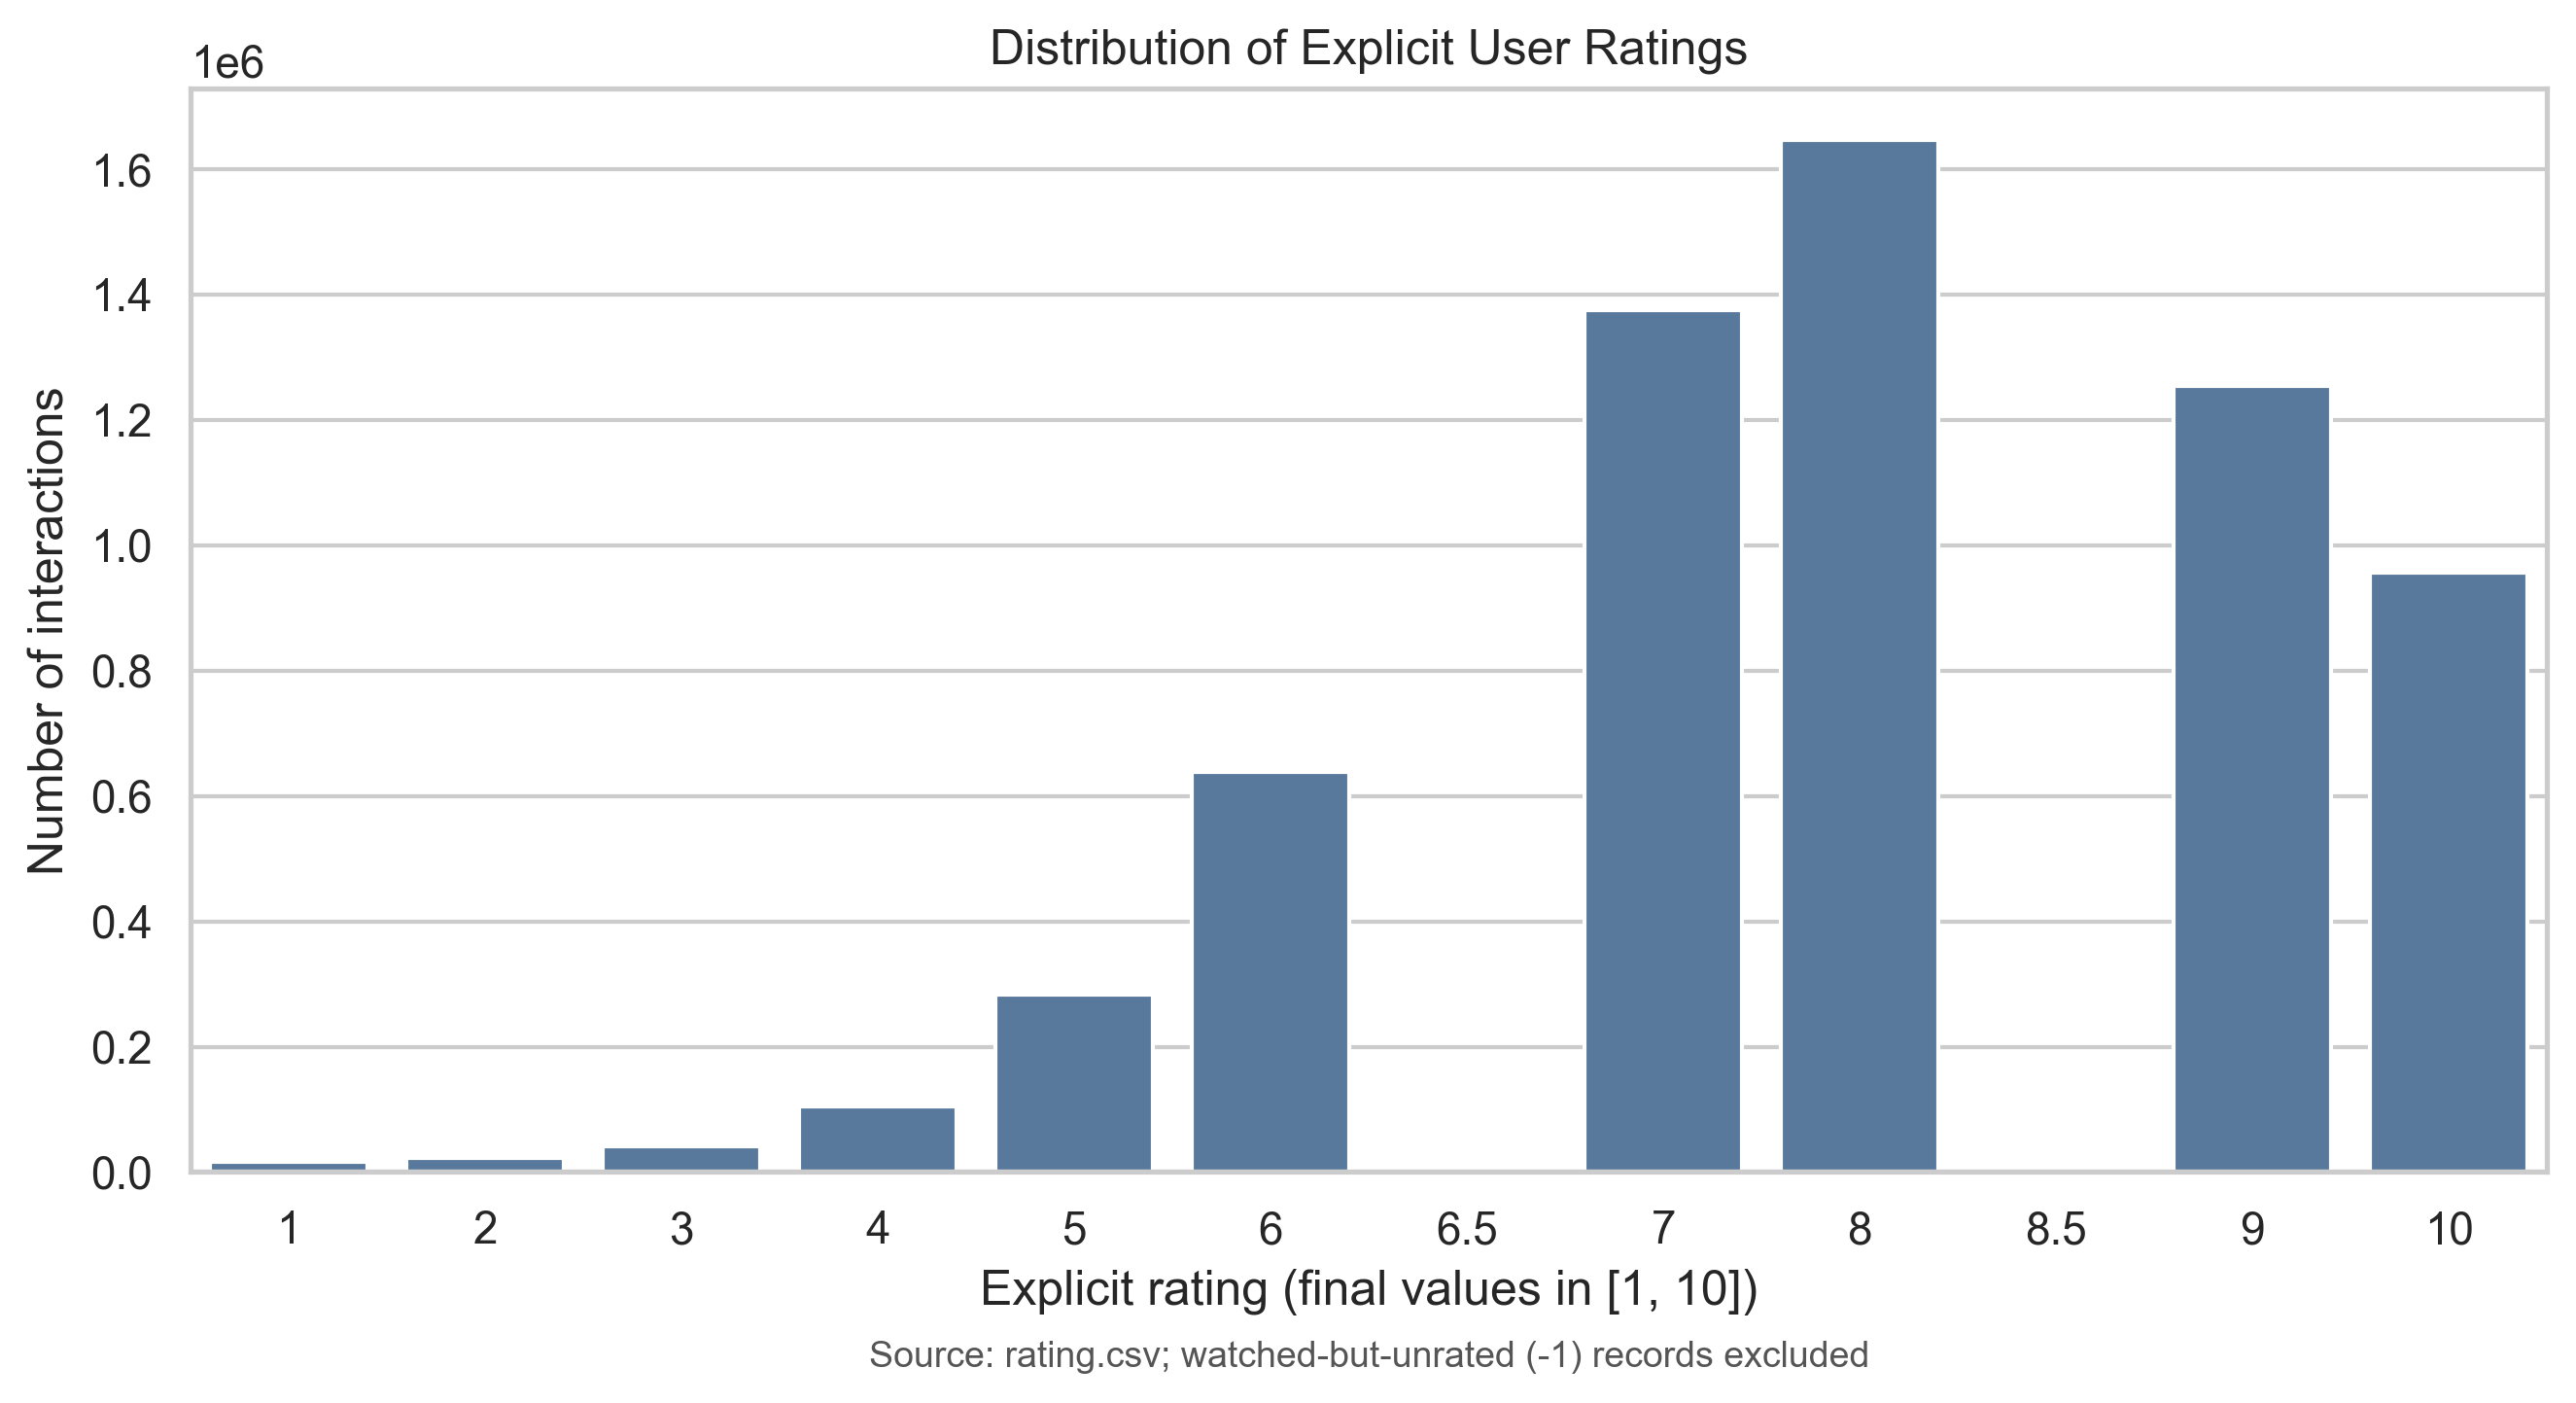
\includegraphics[width=0.92\linewidth]{figures/eda_rating_distribution.png}
  \caption{Distribution of explicit user ratings after excluding watched-but-unrated ($-1$) interactions.}
  \label{fig:rating-distribution}
\end{figure}

Figure~\ref{fig:user-activity} shows the long-tail distribution of ratings per user. The median user has rated 45 anime, whereas the 90th and 99th percentiles are 230 and 640, respectively. This uneven history means that the available collaborative signal differs materially between users. It motivates reporting model coverage and any minimum-interaction rule separately, but it does not justify deleting highly active users as numerical outliers.

\begin{figure}[H]
  \centering
  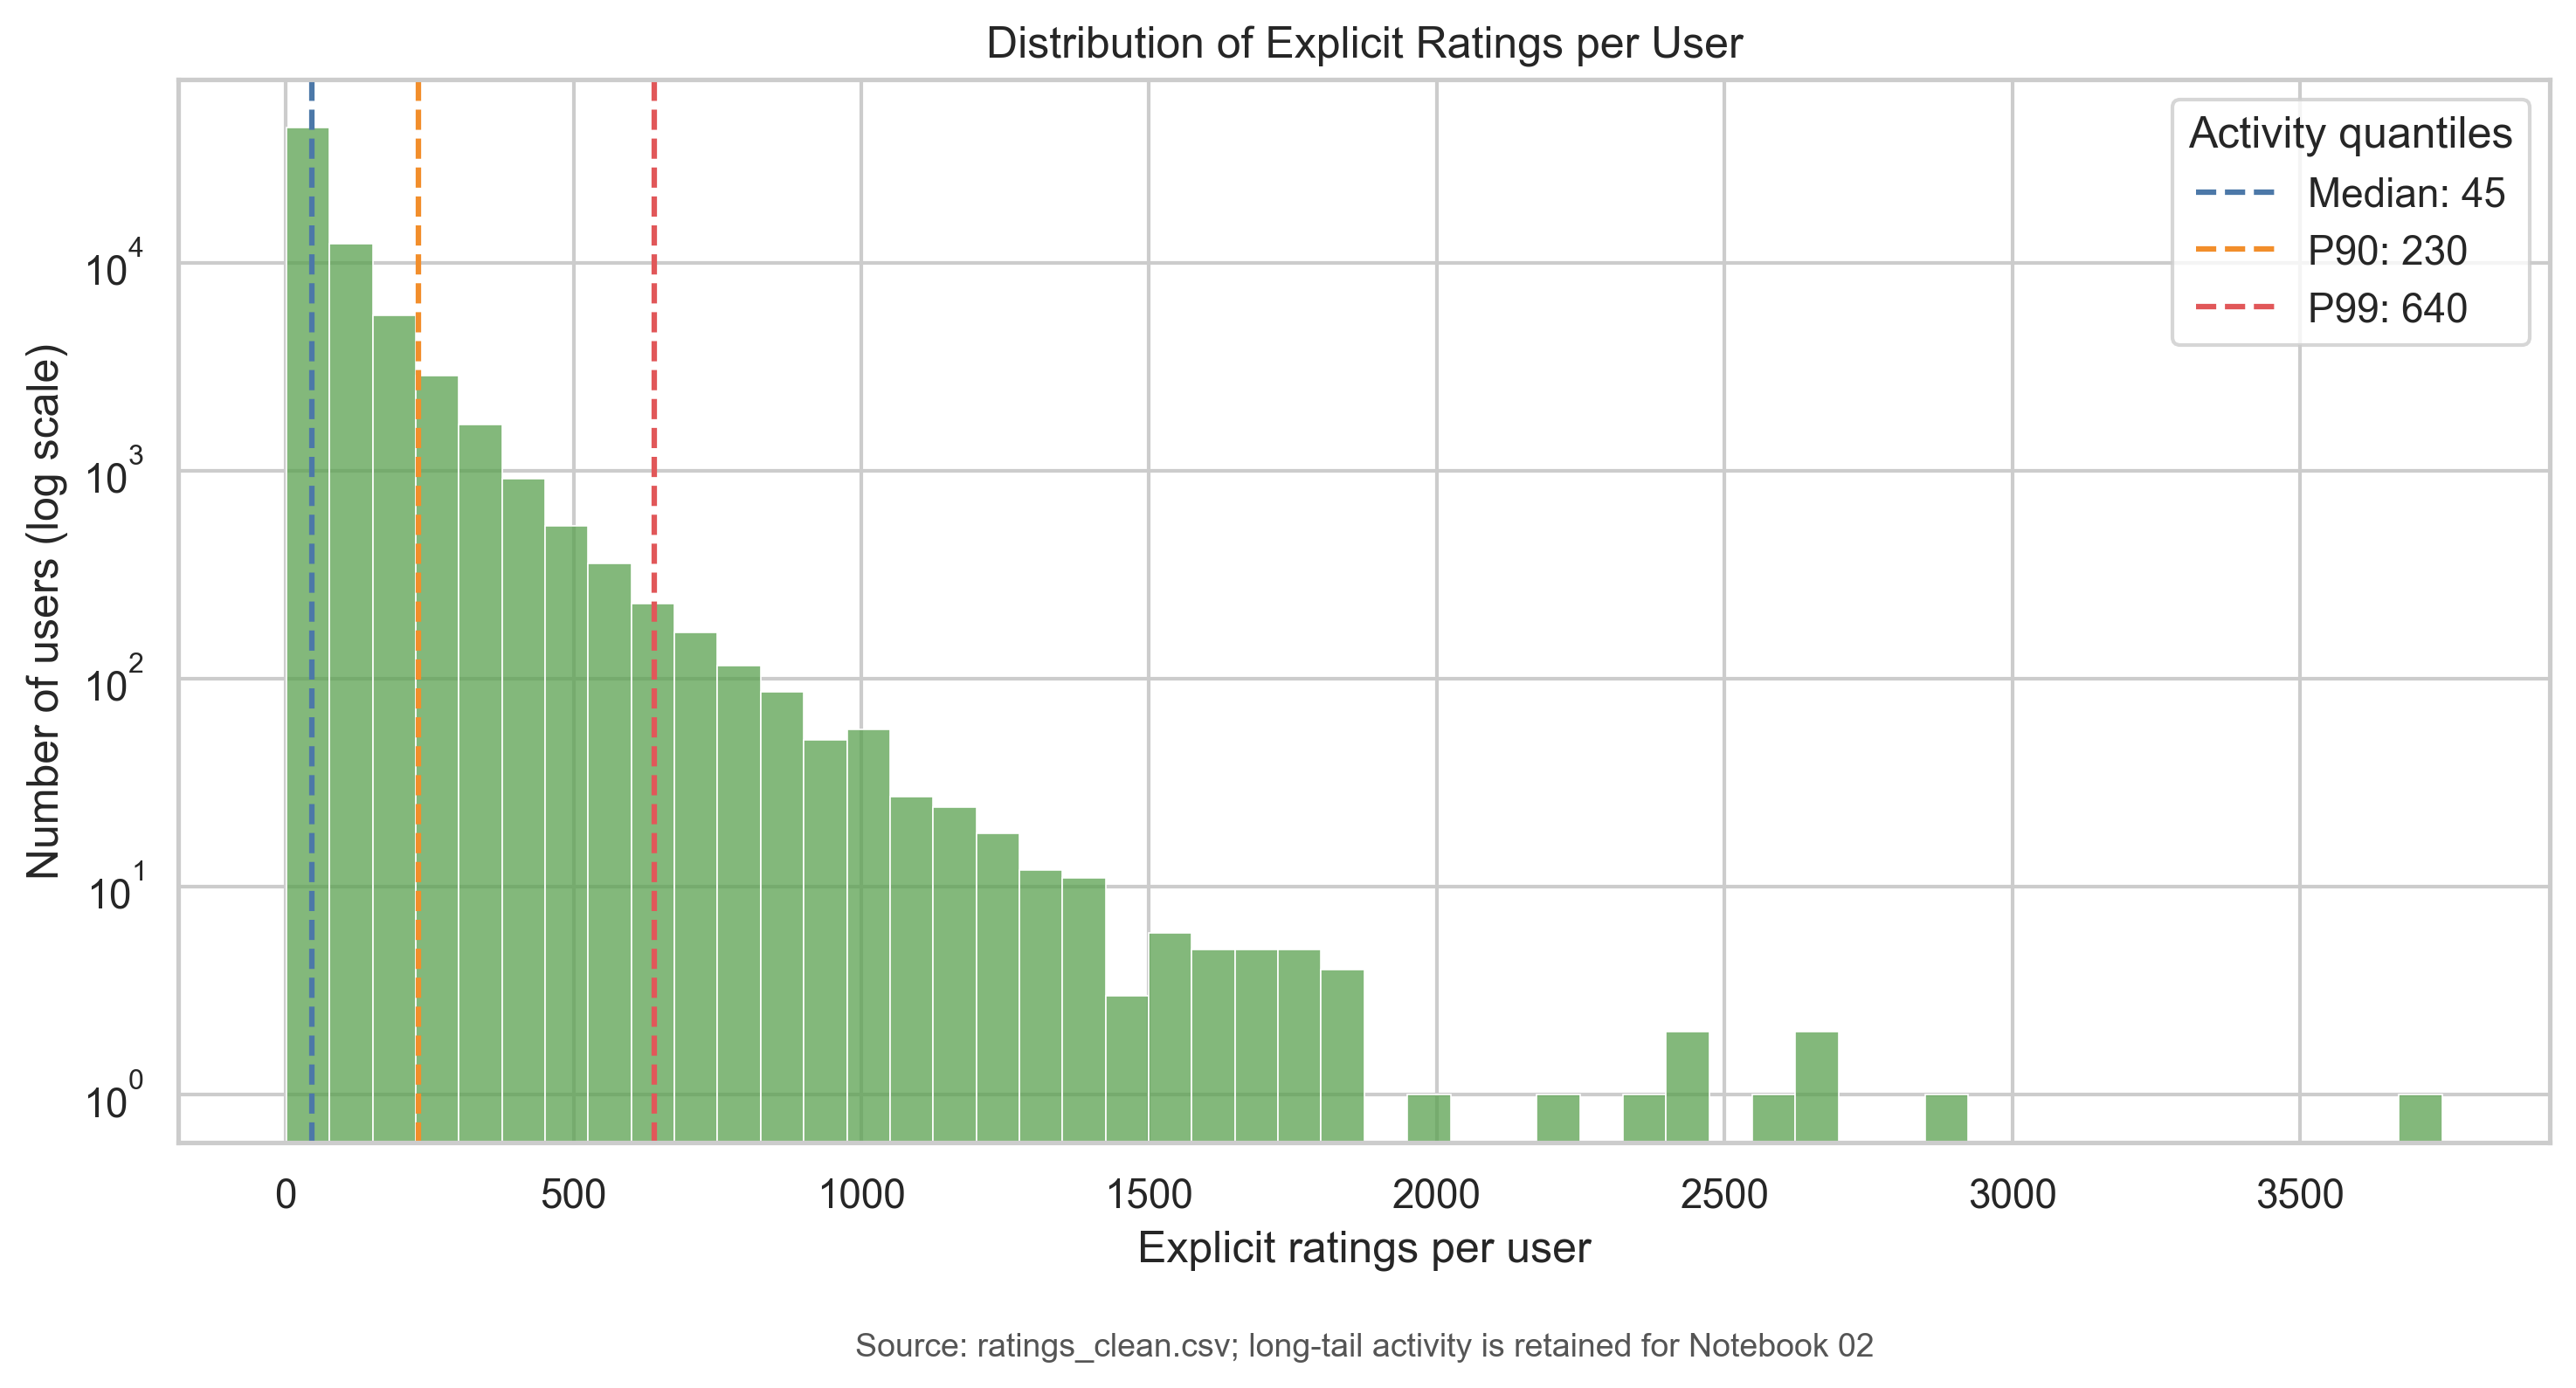
\includegraphics[width=0.92\linewidth]{figures/eda_user_rating_count_distribution.png}
  \caption{Long-tail distribution of explicit-rating counts per user (logarithmic frequency axis).}
  \label{fig:user-activity}
\end{figure}

The 0.9172\% matrix density confirms that most possible user--anime pairs are unobserved. Collaborative filtering is appropriate because it can use shared patterns among observed ratings without converting unknown pairs into zero-valued preferences. Sparsity and the long tail also signal cold-start and popularity-bias risks that qualify later results.

\section{Methodology}
\subsection{Collaborative filtering with SVD}
The system uses the biased SVD implementation in the Surprise library. This form estimates a user's rating for anime $i$ as
\begin{equation}
  \hat{r}_{ui} = \mu + b_u + b_i + q_i^{T}p_u,
\end{equation}
where $\mu$ is the global mean rating, $b_u$ and $b_i$ are user and anime biases, and $p_u$ and $q_i$ are learned latent-factor vectors. The model learns these terms from training ratings by minimising regularised squared error with stochastic gradient descent \parencite{hug2025, koren2009}. Latent factors are inferred preference patterns, not manually assigned genre labels.

The full cleaned dataset was retained as the auditable data baseline. For a resource-aware model run, Notebook 02 used a reproducible random sample of 1,000,000 ratings (seed 42), then iteratively removed users and anime with fewer than five interactions. The final model data comprised 952,497 interactions, 41,370 users, and 5,985 anime. This filter improves the availability of training signal but narrows coverage, so it must not be described as the whole cleaned dataset.

Before final scoring, a bias-only \texttt{BaselineOnly} model was fitted as a benchmark. The SVD search then used a seeded validation split created only from the 80\% outer training data and compared 30, 50, and 100 latent factors. It selected 30 factors (validation RMSE 1.2649, versus 1.2723 and 1.2817); the remaining SVD settings were 20 epochs, learning rate 0.005, regularisation of 0.02, and random state 42. The selected configuration was trained on all 761,997 outer-training ratings and evaluated once on 190,500 held-out ratings. This is lightweight tuning rather than exhaustive hyperparameter optimisation, and the outer test set did not affect configuration selection.

\subsection{Evaluation protocol}
RMSE and MAE compare predicted ratings with the outer holdout's true 1--10 scores. For ranking, predictions were grouped by user and sorted by predicted rating. An item was relevant when its true held-out rating was at least 8. Precision@10 is the fraction of the ten highest-predicted held-out items that are relevant; Recall@10 is the fraction of each eligible user's relevant held-out items recovered in that top ten. Metrics are macro-averaged over 4,802 eligible users who have at least ten test items and at least one relevant test item.

This is \emph{held-out observed-item ranking}, not a ranking experiment over every unseen catalogue item. Of 37,748 test users, 32,911 had fewer than ten test items and 35 had no relevant test item, so they were excluded under the documented protocol rather than given artificial zero recall. For serving, a separate SVD model was refitted on all 952,497 model-data interactions and ranked only anime not already rated by the selected user.

\subsection{Serving model and Top-N recommendation protocol}
The evaluation model is deliberately not used to generate the final displayed recommendations. After the outer-holdout metrics were fixed, a new SVD model with the same configuration was refitted on all 952,497 interactions in \texttt{ratings\_model}. For a user $u$, the serving candidate set contains every anime represented in that model data that $u$ has not already rated. The system predicts $\hat{r}_{ui}$ for each candidate, sorts by predicted rating in descending order (breaking ties by anime ID), and returns the first $N=10$ unseen titles. Thus, the output answers ``which model-scope unseen anime receive the highest estimated preference?''; it does not confirm that the user will watch or rate any title.

Seven users were selected deterministically to make the output inspection reproducible across distinct interaction histories: limited history, developing history, typical history, very active, highly positive, more critical, and broad genre exposure. The user cases are examples of serving behaviour only. They are not additional test folds and are not used to calculate or validate the four evaluation metrics.

\section{Implementation}
The implementation is divided into two reproducible notebooks. Notebook 01 loads the raw CSV files, validates schema and missingness, audits sentinel values and duplicate keys, writes the two cleaned CSV files, and saves the EDA figures. Assertions verify the 1--10 scale, the absence of $-1$, unique user--anime keys, and unique metadata IDs. This notebook intentionally stops before sampling, filtering, splitting, or training.

Notebook 02 reads only those cleaned outputs. It applies the fixed-seed sampling and k-core audit, creates the outer train/test split, benchmarks a bias-only model, tunes the SVD factor count within the outer training data, calculates rating and ranking metrics, and saves evaluation charts. It then refits the selected SVD configuration on the final model data, excludes previously rated anime from each candidate set, joins metadata with fallbacks, and exports ten recommendations per demonstration user. The two-stage design keeps evaluation honest while permitting the recommendation model to use all model-scope interactions.

\section{Results and evaluation}
Table~\ref{tab:metrics} reports the outer-holdout results for the 30-factor SVD selected using only the outer-training data. The bias-only benchmark obtained RMSE 1.2552 and MAE 0.9604; the selected SVD marginally reduced both errors to 1.2551 and 0.9560, respectively. Precision@10 of 0.6397 and Recall@10 of 0.8273 quantify performance only under the stated relevant-rating threshold, eligible-user rule, and observed-item candidate set. They should not be interpreted as full-catalog Top-10 performance.

\begin{table}[H]
  \centering
  \caption{Selected 30-factor SVD outer-holdout evaluation on 952,497 sampled and k-core-filtered interactions (seed 42).}
  \label{tab:metrics}
  \begin{tabular}{lr l}
    \toprule
    \textbf{Metric} & \textbf{Value} & \textbf{Direction} \\
    \midrule
    RMSE & 1.2551 & Lower is better \\
    MAE & 0.9560 & Lower is better \\
    Precision@10 & 0.6397 & Higher is better \\
    Recall@10 & 0.8273 & Higher is better \\
    \bottomrule
  \end{tabular}
\end{table}

Figures~\ref{fig:error-metrics} and \ref{fig:ranking-metrics} make the two evaluation views visible. The error values show the residual scale of individual rating estimates; the ranking measures show retrieval of explicit high ratings within eligible users' held-out observations. Neither visual demonstrates a causal effect or a guarantee that a newly recommended anime will be liked.

\begin{figure}[H]
  \centering
  
\includegraphics[width=0.72\linewidth]{figures/svd_error_metrics.png}
  \caption{SVD rating-prediction error on the outer holdout (lower is better).}
  \label{fig:error-metrics}
\end{figure}

\begin{figure}[H]
  \centering
  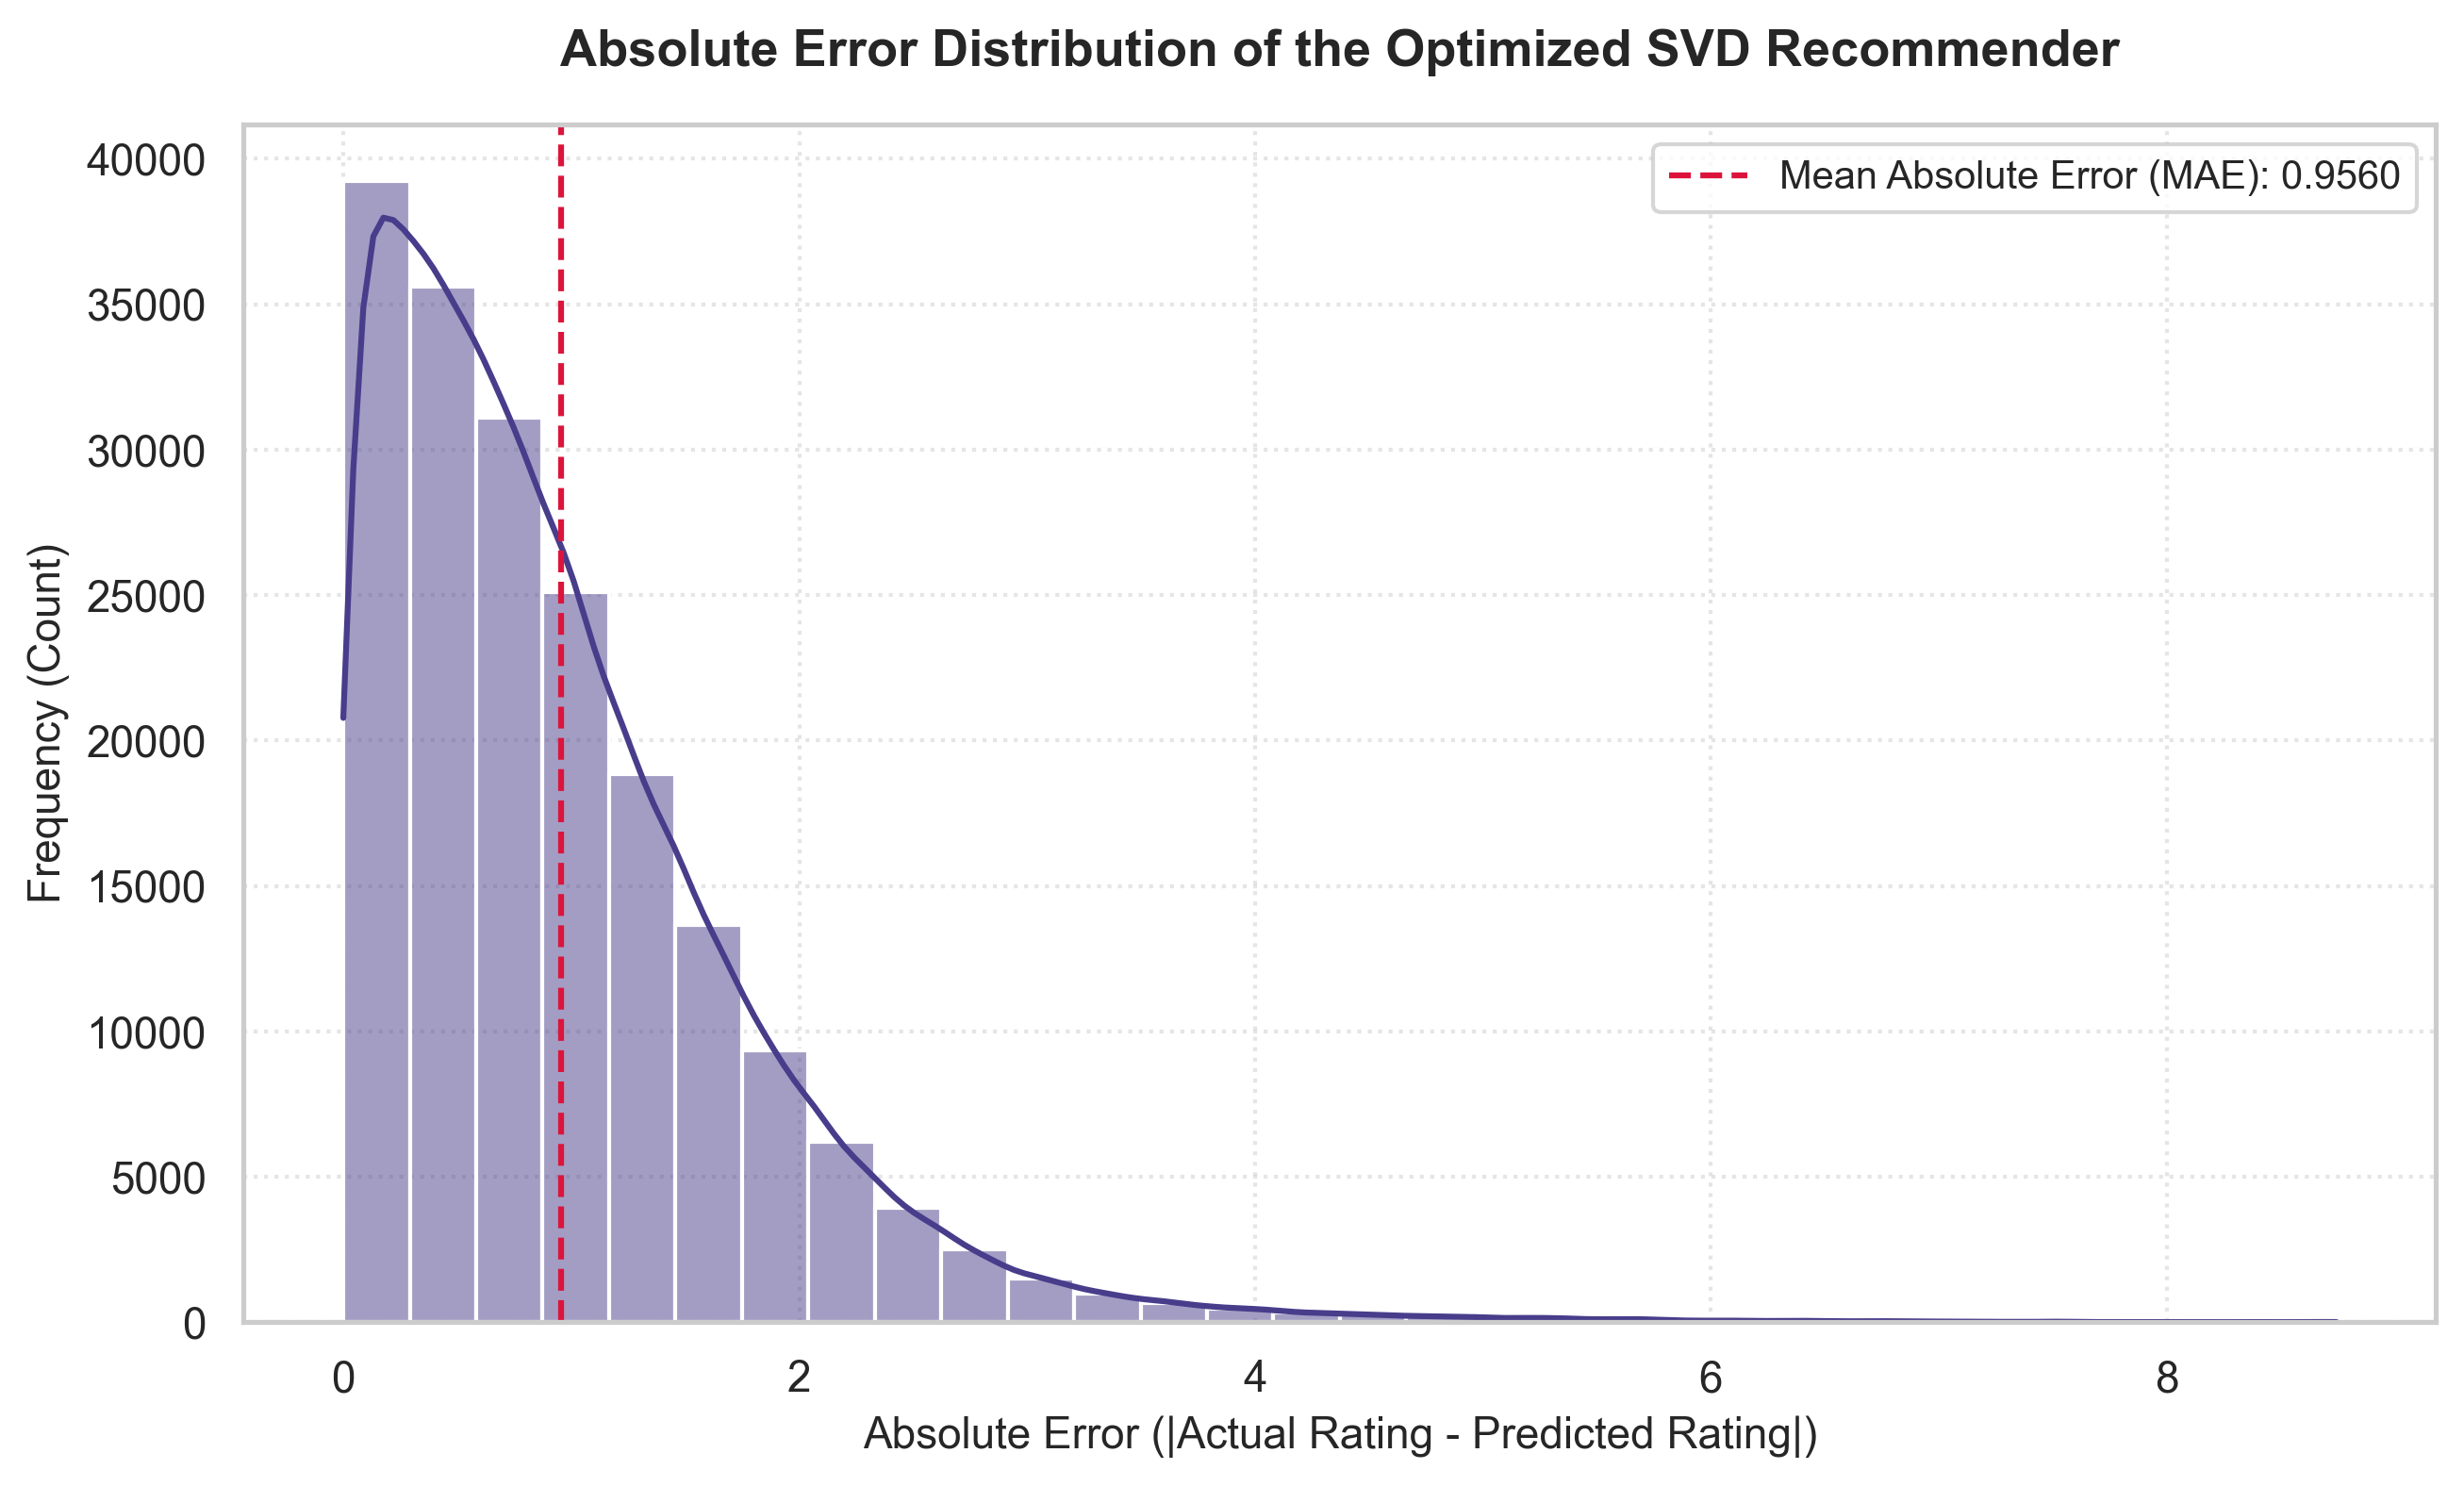
\includegraphics[width=0.82\linewidth]{figures/svd_error_distribution.png}
  \caption{Distribution of absolute prediction errors for the selected SVD model on the outer holdout. The dashed line marks MAE.}
  \label{fig:error-distribution}
\end{figure}

\begin{figure}[H]
  \centering
  
\includegraphics[width=0.72\linewidth]{figures/svd_ranking_metrics_at_10.png}
  \caption{Held-out observed-item ranking metrics at 10 for 4,802 eligible users (higher is better).}
  \label{fig:ranking-metrics}
\end{figure}

\subsection{Case-based Top-N recommendation outputs}
The serving export contains ten unseen anime for each of the seven demonstration users, with title, genre, type, public average rating, and predicted rating. Table~\ref{tab:serving-profiles} describes the interaction histories used to select the cases. The \emph{mean observed rating} and \emph{observed genres} are profile descriptors calculated from \texttt{ratings\_model}; they are not model features added to SVD.

\begin{table}[H]
  \centering
  \caption{Deterministic demonstration profiles for the Top-10 serving outputs.}
  \label{tab:serving-profiles}
  \small
  \begin{tabularx}{\linewidth}{Y r r r r}
    \toprule
    \textbf{Scenario} & \textbf{User ID} & \textbf{Ratings} & \textbf{Mean rating} & \textbf{Genres} \\
    \midrule
    Limited history & 10004 & 5 & 8.00 & 10 \\
    Developing history & 10060 & 10 & 7.70 & 18 \\
    Typical history & 25321 & 33 & 7.79 & 30 \\
    Very active & 42635 & 513 & 6.38 & 43 \\
    Highly positive & 45649 & 121 & 10.00 & 30 \\
    More critical & 24323 & 45 & 1.60 & 31 \\
    Broad genre exposure & 65836 & 255 & 6.26 & 43 \\
    \bottomrule
  \end{tabularx}
\end{table}

The detailed predictions in Appendix~\ref{tab:case-top-ten} illustrate why a single aggregate metric cannot describe every user experience. User \texttt{10004}, with only five retained ratings, receives a highly scored but necessarily less evidence-rich list. User \texttt{42635} has 513 ratings, giving the model substantially more interaction signal, yet its highest estimated preference is 8.8971 rather than a ceiling score. The highly positive profile (user \texttt{45649}) receives ten estimates of 10.0000, while the more critical profile (user \texttt{24323}) has a highest estimate of 5.1974. These are model estimates conditional on observed ratings and the fitted score range, not statements that one user's recommendations are objectively better than another's. The broad-genre user (\texttt{65836}) demonstrates that the list can span several genres, but the latent factors themselves must not be interpreted as named genre dimensions.

Every row in Appendix~\ref{tab:case-top-ten} is an unseen anime at the time of serving. Predicted ratings are rounded to four decimal places for presentation; the full-precision values, metadata, and all ranks are retained in \texttt{outputs/top\_10\_recommendations.csv}. Public \texttt{anime\_average\_rating} is deliberately excluded from that appendix so it cannot be confused with the personalised SVD prediction.

\section{Complete Top-10 serving outputs}
This appendix reports the complete $N=10$ unseen-anime lists exported by the serving model for all seven deterministic demonstration profiles. The lists are descriptive outputs from the refitted serving model, not holdout observations. A predicted rating of 10.0000 is an estimate at the upper bound of the configured 1--10 scale; it is not a verified future rating.

\begingroup
\small
\begin{longtable}{r p{0.64\linewidth} r}
  \caption{Personalised Top-10 unseen-anime predictions for each demonstration profile.}\label{tab:case-top-ten} \\
  \toprule
  \textbf{Rank} & \textbf{Anime title} & \textbf{Predicted rating} \\
  \midrule
  \endfirsthead
  \multicolumn{3}{l}{\small\itshape Table~\ref{tab:case-top-ten} continued} \\
  \toprule
  \textbf{Rank} & \textbf{Anime title} & \textbf{Predicted rating} \\
  \midrule
  \endhead
  \bottomrule
  \endfoot
  \multicolumn{3}{@{}l}{\textbf{Limited history --- user \texttt{10004}}} \\
  \addlinespace[2pt]
  1 & Ginga Eiyuu Densetsu & 9.9322 \\
  2 & Kimi no Na wa. & 9.5840 \\
  3 & Hotaru no Haka & 9.5256 \\
  4 & Gintama': Enchousen & 9.4666 \\
  5 & Aria The Origination & 9.4278 \\
  6 & Gintama' & 9.3549 \\
  7 & Gintama$^\circ$ & 9.3215 \\
  8 & Mushishi Special: Hihamukage & 9.2763 \\
  9 & Gintama Movie: Kanketsu-hen -- Yorozuya yo Eien Nare & 9.2309 \\
  10 & Ping Pong The Animation & 9.2182 \\
  \addlinespace[5pt]
  \multicolumn{3}{@{}l}{\textbf{Developing history --- user \texttt{10060}}} \\
  \addlinespace[2pt]
  1 & Ginga Eiyuu Densetsu & 9.9855 \\
  2 & Gintama$^\circ$ & 9.7026 \\
  3 & Gintama' & 9.5512 \\
  4 & Code Geass: Hangyaku no Lelouch & 9.5019 \\
  5 & Kimi no Na wa. & 9.4868 \\
  6 & Code Geass: Hangyaku no Lelouch R2 & 9.4163 \\
  7 & Nana & 9.3691 \\
  8 & Haikyuu!!: Karasuno Koukou VS Shiratorizawa Gakuen Koukou & 9.3169 \\
  9 & Ping Pong The Animation & 9.3159 \\
  10 & Aria The Origination & 9.3152 \\
  \addlinespace[5pt]
  \multicolumn{3}{@{}l}{\textbf{Typical history --- user \texttt{25321}}} \\
  \addlinespace[2pt]
  1 & Ginga Eiyuu Densetsu & 9.6250 \\
  2 & Gintama$^\circ$ & 9.4408 \\
  3 & Neon Genesis Evangelion & 9.4265 \\
  4 & Fullmetal Alchemist: Brotherhood & 9.3124 \\
  5 & Byousoku 5 Centimeter & 9.2897 \\
  6 & Hunter x Hunter (2011) & 9.2766 \\
  7 & Gintama Movie: Kanketsu-hen -- Yorozuya yo Eien Nare & 9.2697 \\
  8 & Monster & 9.2488 \\
  9 & Gintama': Enchousen & 9.1641 \\
  10 & Kara no Kyoukai 5: Mujun Rasen & 9.1538 \\
  \addlinespace[5pt]
  \multicolumn{3}{@{}l}{\textbf{Very active --- user \texttt{42635}}} \\
  \addlinespace[2pt]
  1 & Ginga Eiyuu Densetsu & 8.8971 \\
  2 & Mushishi & 8.7969 \\
  3 & Toki wo Kakeru Shoujo & 8.6651 \\
  4 & Sword Art Online & 8.6465 \\
  5 & Fullmetal Alchemist: Brotherhood & 8.5818 \\
  6 & Shigatsu wa Kimi no Uso & 8.5690 \\
  7 & Kimi no Na wa. & 8.5641 \\
  8 & Gintama Movie: Kanketsu-hen -- Yorozuya yo Eien Nare & 8.5552 \\
  9 & Shingeki no Kyojin & 8.5115 \\
  10 & Gintama' & 8.4912 \\
  \addlinespace[5pt]
  \multicolumn{3}{@{}l}{\textbf{Highly positive --- user \texttt{45649}}} \\
  \addlinespace[2pt]
  1 & Cowboy Bebop & 10.0000 \\
  2 & Uchuu Kaizoku Captain Harlock & 10.0000 \\
  3 & Carnival Phantasm & 10.0000 \\
  4 & Shouwa Monogatari & 10.0000 \\
  5 & Top wo Nerae 2! Diebuster & 10.0000 \\
  6 & Ore no Imouto ga Konnani Kawaii Wake ga Nai Specials & 10.0000 \\
  7 & Coquelicot-zaka kara & 10.0000 \\
  8 & Bakuman. 2nd Season & 10.0000 \\
  9 & Toriko & 10.0000 \\
  10 & Nurarihyon no Mago: Sennen Makyou & 10.0000 \\
  \addlinespace[5pt]
  \multicolumn{3}{@{}l}{\textbf{More critical --- user \texttt{24323}}} \\
  \addlinespace[2pt]
  1 & Dragon Ball Z & 5.1974 \\
  2 & Sennen Joyuu & 5.0600 \\
  3 & Hotaru no Haka & 4.9261 \\
  4 & Suzumiya Haruhi no Shoushitsu & 4.8688 \\
  5 & Ginga Eiyuu Densetsu & 4.8455 \\
  6 & Gintama': Enchousen & 4.4868 \\
  7 & Kimi no Na wa. & 4.4423 \\
  8 & Kimi ga Nozomu Eien & 4.3804 \\
  9 & Digimon Adventure & 4.3404 \\
  10 & Tengen Toppa Gurren Lagann & 4.2814 \\
  \addlinespace[5pt]
  \multicolumn{3}{@{}l}{\textbf{Broad genre exposure --- user \texttt{65836}}} \\
  \addlinespace[2pt]
  1 & Ghost in the Shell & 10.0000 \\
  2 & Dragon Ball Z & 9.3731 \\
  3 & Gintama': Enchousen & 9.3722 \\
  4 & Nana & 9.1538 \\
  5 & Naruto Movie 1: Dai Katsugeki!! Yuki Hime Shinobu Houjou Dattebayo! & 9.1357 \\
  6 & Neon Genesis Evangelion: The End of Evangelion & 8.9466 \\
  7 & Rurouni Kenshin: Meiji Kenkaku Romantan - Tsuioku-hen & 8.9105 \\
  8 & K-On! & 8.8223 \\
  9 & Kino no Tabi: The Beautiful World & 8.7995 \\
  10 & Mahou Shoujo Madoka$^\star$Magica Movie 2: Eien no Monogatari & 8.6599 \\
\end{longtable}
\endgroup

\section{Conclusion and lessons learned}
This project produced a reproducible anime recommender based on explicit ratings and biased SVD. The data audit preserves the meaning of watched-but-unrated interactions, removes duplicate user--anime ambiguity, and exposes the sparse, positively skewed, long-tail structure that affects recommendation quality. On the documented sampled and filtered outer holdout, the validation-selected 30-factor model achieved RMSE 1.2551, MAE 0.9560, Precision@10 0.6397, and Recall@10 0.8273.

As students who had previously learned recommender-system ideas mainly in theory, our first important lesson was that a model cannot compensate for an unclear definition of the data. At first, it is tempting to regard every row in a ratings file as a training example and to begin fitting SVD immediately. Working with the dataset showed why that is unsafe: the value $-1$ means ``watched but not rated,'' not a low preference, and repeated user--anime pairs do not directly form one matrix cell. We learned to ask what each value represents before applying a transformation, to validate the result with assertions, and to keep an audit trail of every removed or merged row. In other words, data cleaning is not only a technical preparation step; it is a modelling decision that determines the meaning of the signal learned by the recommender.

The second lesson was to connect the mathematical model to the actual structure of the data. In class, collaborative filtering and SVD can appear as a compact equation with latent factors. During the project, the sparse matrix, strongly positive ratings, and unequal user histories made the practical consequences visible. Missing ratings are unknown rather than zero, a user with five ratings provides much less evidence than a user with hundreds, and a high predicted score must be interpreted against a scale on which many users already give high scores. We therefore learned that latent factors are useful learned patterns rather than automatically interpretable genres, and that a reasonable baseline needs limitations such as cold start, popularity imbalance, and incomplete coverage to be reported alongside its predictions.

The third lesson concerned experimental design and evaluation. We learned that obtaining a numerical score is not the same as demonstrating a useful recommender. The outer train/test split has to be created before fitting so that held-out ratings do not influence the model, and the final serving model should be refitted only after the evaluation result is fixed. RMSE and MAE taught us about the error of estimated ratings, while Precision@10 and Recall@10 taught us a different question: whether relevant held-out items appear near the top of a ranked list. Implementing both views made clear that metrics answer only the question defined by their protocol. In this project, ranking is measured over held-out observed items for eligible users, so it must not be described as full-catalog Top-10 performance or as a guarantee that a user will like every suggested anime.

Finally, the project taught us the value of reproducible teamwork. Fixed random seeds, saved cleaned files, documented sampling and k-core filtering, notebook-generated figures, and cross-checking the report against exported artifacts made it possible to explain where each result came from. These practices were more demanding than simply running a notebook once, but they helped us distinguish the full cleaned dataset from the smaller model dataset and avoid claims beyond the evidence. Overall, the project moved our understanding from ``how to train an SVD recommender'' to ``how to define, build, test, interpret, and communicate a recommender responsibly.'' The current model is a baseline rather than a finished product, but the lessons from data semantics, sparse-data behaviour, honest evaluation, and reproducibility provide a practical foundation for future work such as stronger model comparison, temporal validation, and cold-start solutions.


\printbibliography[title={References}]

\end{document}
